\documentclass{article}

% if you need to pass options to natbib, use, e.g.:
% \PassOptionsToPackage{numbers, compress}{natbib}
% before loading nips_2017
%
% to avoid loading the natbib package, add option nonatbib:
% \usepackage[nonatbib]{nips_2017}

\usepackage[final]{nips_2017}

% to compile a camera-ready version, add the [final] option, e.g.:
% \usepackage[final]{nips_2017}
\usepackage{subfigure}
\usepackage[utf8]{inputenc} % allow utf-8 input
\usepackage[T1]{fontenc}    % use 8-bit T1 fonts
\usepackage{hyperref}       % hyperlinks
\usepackage{url}            % simple URL typesetting
\usepackage{booktabs}       % professional-quality tables
\usepackage{amsfonts}       % blackboard math symbols
\usepackage{nicefrac}       % compact symbols for 1/2, etc.
\usepackage{microtype}      % microtypography
\usepackage{cite}
\usepackage{amsmath}
\usepackage{graphicx} 
\usepackage{listings}

\usepackage{algorithm}  
\usepackage{algpseudocode}  
\usepackage{amsmath}  
\renewcommand{\algorithmicrequire}{\textbf{Input:}}  % Use Input in the format of Algorithm  
\renewcommand{\algorithmicensure}{\textbf{Output:}} % Use Output in the format of Algorithm  

\hypersetup{colorlinks,linkcolor={blue},citecolor={blue},urlcolor={blue}}  

\title{CS150A Database \\Course Project}

% The \author macro works with any number of authors. There are two
% commands used to separate the names and addresses of multiple
% authors: \And and \AND.
%
% Using \And between authors leaves it to LaTeX to determine where to
% break the lines. Using \AND forces a line break at that point. So,
% if LaTeX puts 3 of 4 authors names on the first line, and the last
% on the second line, try using \AND instead of \And before the third
% author name.

\author{
  Student 1: Entropy-Fighter\\
  ID: 2020533xxx\\
  \texttt{xxxx@shanghaitech.edu.cn} \\
  %% examples of more authors
   \And
  Student 2: Chenyh\\
  ID: 2020533xxx\\
  \texttt{xxxx@shanghaitech.edu.cn}
}

\begin{document}
% \nipsfinalcopy is no longer used

\maketitle

\begin{abstract}
This project is about using ML to predict student performance. In the project, we follow the 5 steps given by the instructor and use PySpark to improve the efficiency.
Our final RMSE on valid data in "test.csv" is close to 0.3539.
% Compared with developing a novel machine learning algorihtm, building a machine learning system is less theoretical but more engineering, so it is important to get your hands dirty. To build an entire machine learning system, you have to go through some essential steps. We have listed 5 steps which we hope you to go through. Read the instructions of each section before you fill in. You are free to add more sections. \\
% If you use PySpark to implement the algorithms and want to earn some additional points, you should also report your implementation briefly in the last section.
\end{abstract}

\section{Explore the dataset}
%\textcolor{cyan}{Instruction: \\
% Explore the given dataset, report your findings about the dataset. You should not repeat the information provided in the 'Data Format' section of project.pdf. Instead, you can report the data type of each feature, the distribution of different values of some important features(maybe with visualization), is there any missing value, etc}\\\\
% \textbf{Your work below:}\\
\subsection{Getting basic information by reading the dataset}
In our data set, we can find that the total 19 features can be separated into 2 types: categorical features like "Student Name", and numerical features like 
"Step Duration".

As for the structure of data, we find "Problem Hierarchy" can be separated into "Problem Unit" and "Problem
Section". We also find one row can have more than one KC, which are connected by $\sim\sim$. Therefore, we can separate the KCs by $\sim\sim$. "Opportunity"'s situation is the same with "KC".

As for the missing values, in "train.csv", we find some values of "Correct Step Duration", "Error Step Duration", "KC" and "Opportunity" are NaN. In "test.csv", we find that values of "Step Start Time", "First Transaction
Time", "Correct Transaction Time", "Step End Time", "Step Duration", "Correct Step Duration", "Error Step Duration", "Correct First Attempt", "Incorrects", "Hints" and "Corrects" are missing.
\subsection{Data type of each feature}
\quad Using dtypes, we get the following results.
\begin{figure}[h]
	\centering
	\subfigure[type]
	{
		\begin{minipage}[b]{.4\linewidth}
		\centering
		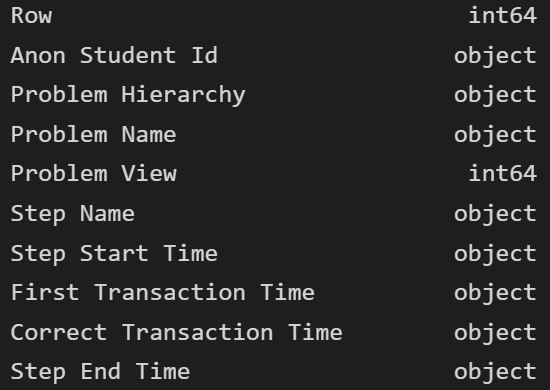
\includegraphics[width = 4cm]{type1.JPG}
		\end{minipage}
	}
	\subfigure[type]
	{
		\begin{minipage}[b]{.4\linewidth}
		\centering
		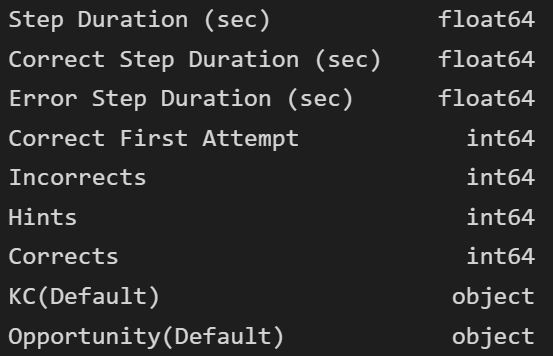
\includegraphics[width = 4cm]{type2.JPG}
		\end{minipage}
	}
\end{figure}
\subsection{Visulization of some statistics}
From the figure below, we can find that if the step duration is long, the CFA tend to be incorrect.
\begin{figure}[h]
	\centering
	{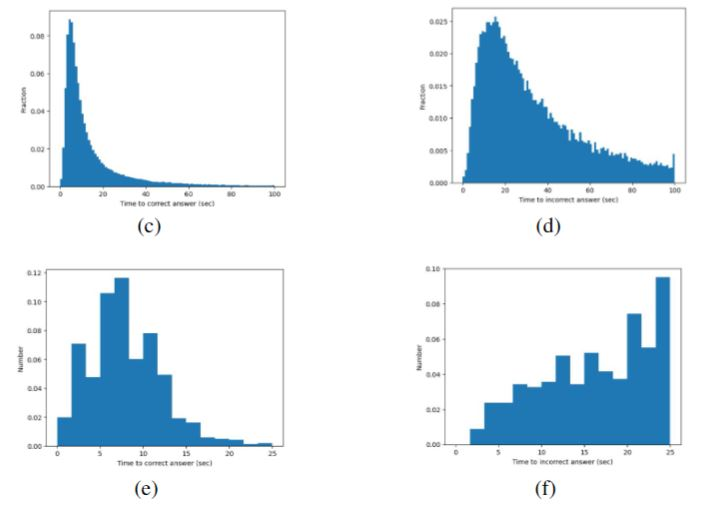
\includegraphics[width=10cm]{5.JPG}}
\end{figure}

\section{Data cleaning}
% \textcolor{cyan}{Instruction: \\
% Some people treat data cleaning as a part of feature engineering, however we separate them here to make your work clearer. In this section, you should mainly deal with the missing values and the outliers. You can also do some data normalization here.}\\\\
% \textbf{Your work below:}\\
In this section, firstly, we remove some meaningless NaN or replace some NaN to 0 for easier caluculation. Then, we make sure every row is unique and drop duplicates. The outlier is another thing that we need to consider.
We do a easy detection to check whether there are some singular values which are inconsistant with the normal values.

After doing these steps, we simplify the data set for following sections according to our needs. As is introduced in section 1, many column values are missing in "test.csv". Therefore, we consider them useless for this project(maybe few features are meaningful, but we don't consider them for the convenience) 
We remove the following columns in "train.csv": ["Row", "Step Start Time", "First Transaction Time", 
"Correct Transaction Time", "Step End Time", "Step Duration (sec)", 
"Correct Step Duration (sec)", "Error Step Duration (sec)", 
"Incorrects", "Hints", "Corrects"]
\section{Feature engineering}
% \textcolor{cyan}{Instruction: \\
% In this section, you should select a subset of features and transform them into a data matrix which can be feed into the learning model you choose. Report your work with reasons.}\\\\
% \textbf{Your work below:}\\
This part is very important for lowering the RMSE. In the data cleaning part, we have removed some irrelevant features. In this part, we modify some categorical features and add some CFARs as new features.
\subsection{Feature modifications}
Firstly, we separate "Problem Hierarchy" into "Problem Unit" and "Problem Section" according to our findings in data exploration. 
Secondly, we should compress the information of "KC" and "Opportunity". The data format of "KC" is like "String$\sim\sim$String$\sim\sim$String", and the data format of "Oppportunity" is like "Integer$\sim\sim$Integer$\sim\sim$Integer", 
which are too complex. We write 2 functions to simplify them: getKCCount(kcs) and getOpportunityAverage(oppo). The function names give good explanation of what we do. 
We use these 2 functions' results to replace the orginal 2 columns' values.
\subsection{Converting categorical features to numerical ones}
As is shown in data exploration section, we have both categorical features and numerical features. In order to better fit the model, we need to convert categorical features to numerical ones. 
Therefore, we need to do some operations on the following columns: ["Anon Student Id", "Problem Name", 
"Problem Unit", "Problem Section", "Step Name"]. We should do the operations on the union of train set and test set, otherwise we would have 2 different conversions. We use python's dictionary for our naiive conversion. We assign values starting from 0 to different objects. 
\subsection{Adding new features}
To better predict the CFA, we calculate different kinds of Correct First Attempt Ratio(CFAR) and add them as new features(We get this idea from the paper: [2010]Feature Engineering and Classifier Ensemble for KDD Cup 2010, Hsiang-Fu Yu). The formula of CFAR is shown below.
$$ featureX~CFAR = \frac{number~of~rows~with~featureX~=~xid~and~CFA~=~1}{number~of~rows~with~featureX~=~xid} $$
By the above formula, we write the function getCFARTemplate() and calculate "Student CFAR", "Problem CFAR", "Unit CFAR", "Section CFAR", "Step CFAR" and "KC CFAR", since we assume these "featureX" like "student" and "problem" are relevant to the CFA.
\section{Learning algorithm}
% \textcolor{cyan}{Instruction: \\
% In this section, you should describe the learning algorithm you choose and state the reasons why you choose it.}\\\\
% \textbf{Your work below:}\\
After reading some papers and other people's previous work, we decide to choose one best learning algorithm among the following methods. 

\begin{itemize}
  % Tree models where the target variable can take a discrete set of values are called classification trees; in these tree structures, leaves represent class labels and branches represent conjunctions of features that lead to those class labels.
  \item DecisionTreeClassify: A Decision tree is a tree structure, where each internal node denotes a test on an attribute, each branch represents an outcome of the test, and each leaf node (terminal node) holds a class label. 
  A tree can be “learned” by splitting the source set into subsets based on an attribute value test. This process is repeated on each derived subset in a recursive manner called recursive partitioning.
  \item LGBMClassify: Light GBM is a gradient boosting framework that uses tree based learning algorithm. While other algorithms trees grow horizontally, LightGBM algorithm grows vertically meaning it grows leaf-wise and other algorithms grow level-wise. LightGBM chooses the leaf with large loss to grow. It can lower down more loss than a level wise algorithm when growing the same leaf.
  \item XGBoostClassify: In this alogorithm, decision trees are created in sequential form. Weights play an important role in XGBoost. Weights are assigned to all the independent variables which are then fed into the decision tree which predicts results. The weight of variables predicted wrong by the tree is increased and these variables are then fed to the second decision tree. These individual classifiers then ensemble to give a strong and more precise model.
  \item RandomForestClassify: Random forest computes on multiple decision trees and involves the bagging theory. Random Forest has multiple decision trees as base learning models. We randomly perform row sampling and feature sampling from the dataset forming sample datasets for every model.
  \item RandomForestRegression: The principles are the same with RandomForestClassify, but we use regressor rather than classifier.
  \item MLPRegression: Neural networks can sometimes solve complex problems in machine learning. And in this semester, we learn the multi layer perceptron in course CS181, so we want to use mlpregressor in sklearn to have a try.
  \item AdaBoostRegression: What Adaptive Boosting does is that it builds a model and gives equal weights to all the data points. It then assigns higher weights to points that are wrongly classified. Now all the points which have higher weights are given more importance in the next model. It will keep training models until and unless a lowe error is received.
\end{itemize}
We feed training data into these models, then predict the CFA of testing data. Finally, we compare our prediction with the correct answers and calculate RMSE. The RMSE results of the above methods are shown below.
\begin{figure}[h]
	\centering
	{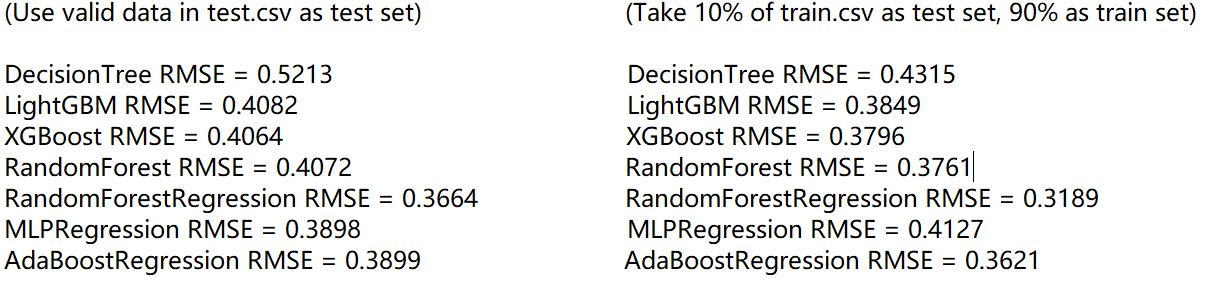
\includegraphics[width=12cm]{result.JPG}}
\end{figure}

It is obvious that RandomForestRegression has best performance among all these methods. We explain our possible reasons below.

Every decision tree has high variance, but when we combine all of them together in parallel then the resultant variance is low as each decision tree gets perfectly trained on that particular sample data and hence the output doesn't depend on one decision tree but multiple decision trees. 
The basic idea behind RandomForestRegression is to combine multiple decision trees in determining the final output rather than relying on individual decision trees. The averaging idea improves the prediction
accuracy and controls over-fitting.
\section{Hyperparameter selection and model performance}
% \textcolor{cyan}{Instruction: \\
% In this section, you should describe the way you choose the hyperparameters of your model, also compare the performance of the model with your chosen hyperparamters with models with sub-optimal hyperparameters}\\\\
% \textbf{Your work below:}\\
In this section, we use function GridSearchCV() as our method to tune the hyper parameters and find the best ones. It is a brute force way, trying all possible cases in a range. Even though it costs a lot of time, it is quite easy to use. 
We tune the following 3 hyperparameters of RandomForestRegression: n\_estimators, max\_depth and max\_leaf\_nodes. The best parameters among our range is shown below.
\begin{itemize}
  \item n\_estimators: 190 in range(50, 200, 10)
  \item max\_depth: 15 in range(5, 20)
  \item max\_leaf\_nodes: 500 in [5, 50, 500, 5000]
  \item original RMSE: 0.3664
  \item best RMSE: 0.3539
\end{itemize}
Due to the tight time, our range is small and the number of hyperparameters is small. Therefore, the best result may be locally optimal, but not globally optimal. No matter whether the result is optimal, it truly gives us a good improvement on RMSE.
\section{PySpark implementation (optional)}
We do the PySpark implementation in Feature Engineering. Spark is a distributed processing method, which is an expert at tackling large-data-size problems. 

In our project, we use pyspark to accelerate the preprocessing part(Feature Engineering), improving the efficiency. 
First, we set the pyspark environment and use SparkSession.builder.getOrCreate() to create the spark. Then we use spark to get our training data and testing data.
\begin{lstlisting}
  os.environ['PYSPARK_PYTHON'] = sys.executable
  os.environ['PYSPARK_DRIVER_PYTHON'] = sys.executable
  spark = SparkSession.builder.getOrCreate()
  training_set = spark.read.csv(xxx)
  testing_set = spark.read.csv(xxx)
\end{lstlisting}
Our implementation mostly use the udf function from pyspark.sql.functions. The general
pyspark implementation is shown below in the template.
\begin{lstlisting}
  @udf(returnType = xxx)
  def functionTemplate():
    xxxxx
\end{lstlisting}
We have 20000+ rows in the training data, which means doing operations on the column is slow.
We first write the basic column operation function, then we need to convert them to the user define function in pyspark. 
The most easy way is to use "@" in python, we only need to add "@udf" above our written function.
Every time we call the function, it uses spark to accelerate.
\end{document}
